\documentclass[11pt,a4paper]{report}
\usepackage[utf8]{inputenc}
\usepackage[english]{babel}
\usepackage[T1]{fontenc}
\usepackage{amsmath}
\usepackage{amsfonts}
\usepackage{amssymb}
\usepackage{makeidx}
\usepackage{graphicx}
\usepackage{float}
\usepackage{lmodern}
\usepackage{tikz}
\usetikzlibrary{intersections}
\usetikzlibrary{optics}
\usetikzlibrary{positioning}
\usepackage{pgfplots}
\usetikzlibrary{calc}
\usepackage{geometry}
\geometry{hmargin=2cm,vmargin=2cm}
\usepackage{fancybox}
\usepackage{xcolor}
\usepackage{mathtools}
\usepackage{enumitem}
\usepackage{tcolorbox}
\usepackage{colortbl}
\usepackage{fancybox}
\tcbuselibrary{most}
\usepackage{pifont}
\usepackage{caption}
\usepackage{subcaption}
\usepackage{eso-pic}
\usepackage{nicematrix}
\usepackage{multicol}
\usepackage{booktabs}
\usepackage{svg}
\usepackage{derivative}
\usepackage{wrapfig}
\usepackage{stmaryrd}
\usepackage{biblatex} %Imports biblatex package %Import the bibliography file
\addbibresource{references.bib}
\author{Andrea}
\setlength{\columnseprule}{0.001 cm}
\setlength{\columnsep}{1cm}
\renewcommand{\thesection}{\Roman{section}}
\renewcommand{\thesubsection}{\arabic{subsection}}
\renewcommand{\thesubsubsection}{\alph{subsubsection}}
\usepackage{amsmath}
\colorlet{shadecolor}{cyan!15}
\usepackage{fancyhdr}
\usepackage{etoolbox}
\renewcommand{\headrulewidth}{0pt}
\usepackage[export]{adjustbox}
\pagestyle{fancy}
\fancyhf{}
\rhead{\textcolor{black}{\today}}
\lhead{\colorbox{lightgray}{%
\makebox[\dimexpr\linewidth][l]{\color{black}%
\includegraphics[height=1.5\baselineskip,valign=c]{ENS.png}
\hspace*{0.3cm} ENS / 
}%
}} 
\rfoot{}
\fancyfoot[C]{\thepage} 
\newlength{\tabcont}
\setlength{\parindent}{0.0in}
\setlength{\parskip}{0.05in}
\begin{document}
\begin{titlepage}
    \AddToShipoutPictureBG*{
        \begin{tikzpicture}[overlay,remember picture]
            \draw [line width=3pt]
            ($ (current page.north west) + (2cm,-2.0cm) $)
            rectangle
            ($ (current page.south east) + (-2cm,1.8cm) $);
            \draw [line width=1pt]
            ($ (current page.north west) + (2.15cm,-2.15cm) $)
            rectangle
            ($ (current page.south east) + (-2.15cm,1.95cm) $);
        \end{tikzpicture}
    }
    \begin{center}
        \begin{figure*}
            \begin{center}
                \vspace*{2cm}
            \end{center}
        \end{figure*}
        \rule{14cm}{2pt}\vspace{.7cm}

        \textbf{Experimental report}

        \vspace{.5cm}
        \rule{14cm}{2pt}\vspace{1cm}
        \vspace{1.5cm}

        \large Bryan Gerard,
        Andrea Combette
        \vspace{1cm}
    \end{center}
\end{titlepage}

\newpage
\tableofcontents
\newpage
\begin{multicols*}{2}
    \chapter{Introduction}
    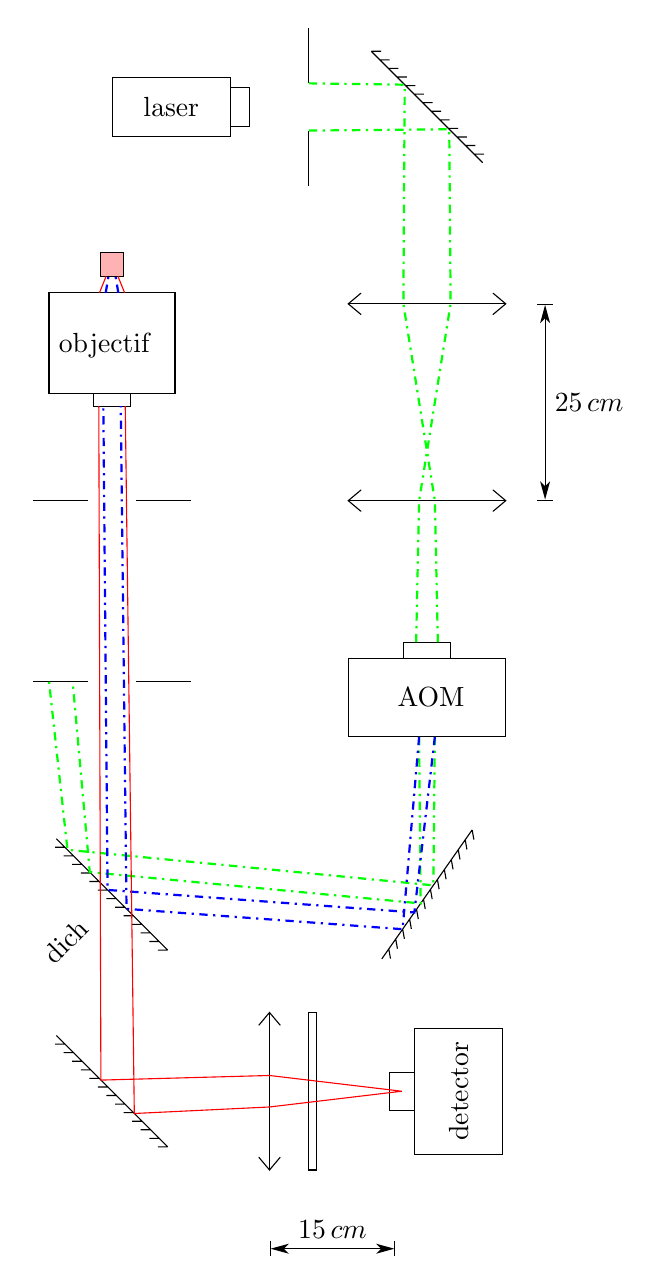
\begin{tikzpicture}[use optics]
        \node[halogen lamp] (quartz iode) at (0,0) {laser};
        \node[slit,right=0.75cm of quartz iode, slit height = 0.3] (fente) {};
        \node[mirror, right=1.5cm of fente, rotate = 45] (M) {};
        \node[lens,rotate = 90] (L) at ($(M)+(0,-2.5cm)$) {};
        \node[lens,rotate = 90] (L2) at ($(L)+(0,-2.5cm)$) {};
        \node[generic optics io,io aperture shift= 0, rotate = 90, io body aspect ratio=0.5, io body height=2cm, io aperture height=0.3, io aperture width=0.1, label={[label distance=-1.6cm,text depth=-1ex,]:AOM}] (AOM) at ($(L2)+(0,-2.5cm)$)  {};
        \node[mirror, rotate = -35] (M2) at ($(AOM)+(0,-2.5cm)$){};
        \node[mirror, rotate = -135, label={[label distance=.4cm,text depth=-1ex,rotate = 45]left:dich}] (Dichro) at ($(M2)+(-4cm,0cm)$){};
        \node[slit, slit height = 0.3, rotate = 90] (fente2) at ($(Dichro)+(0,2.7cm)$){};
        \node[slit, slit height = 0.3, rotate = 90] (fente3) at ($(Dichro)+(0,5cm)$){};
        \node[generic optics io,io aperture shift= 0, rotate = -90, io body aspect ratio=0.8, io body height=1.6cm, io aperture height=0.3, io aperture width=0.1, label={[label distance=-1.6cm,text depth=-1ex,]:objectif}] (objectif) at ($(Dichro)+(0,7cm)$) {};
        \node[fill=red!30][thick optics element, object aspect ratio = 1, object height = 0.3cm](diam) at ($(Dichro)+(0,8cm)$) {};
        \node[mirror, rotate = -135] (M3) at ($(Dichro)+(0cm,-2.5cm)$){};
        \node[lens,] (L3) at ($(M3)+(2cm,0cm)$) {};
        \node[heat filter,right=0.5cm of L3] (AC) {} ;
        \node[generic optics io,io aperture shift= 0, rotate = -180, io body aspect ratio=0.7, io body height=1.6cm, io aperture height=0.3, io aperture width=0.2, label={[text depth=-1ex,rotate = 90]center:detector}] (detector) at ($(L3)+(2.4cm,0cm)$) {};

        south
        \draw[thick,dash dot,green] (fente.slit north) -- ($(M.north)!0.3!(M.south)$) -- ($(L.north)!0.35!(L.south)$) -- ($(L2.north)!0.55!(L2.south)$) -- ($(AOM.aperture north east)!0.73!(AOM.aperture south east)$)
        (fente.slit south) -- ($(M.north)!0.7!(M.south)$) -- ($(L.north)!0.65!(L.south)$) -- ($(L2.north)!0.45!(L2.south)$) -- ($(AOM.aperture north east)!0.27!(AOM.aperture south east)$)
        ($(AOM.body north west)!0.55!(AOM.body south west)$) --  ($(M2.north)!0.43!(M2.south)$) -- ($(Dichro.north)!0.90!(Dichro.south)$) -- ($(fente2.south)!0.90!(fente2.north)$)
        ($(AOM.body north west)!0.45!(AOM.body south west)$) -- ($(M2.north)!0.57!(M2.south)$) -- ($(Dichro.north)!0.70!(Dichro.south)$) -- ($(fente2.south)!0.75!(fente2.north)$);

        \draw[thick,dash dot,blue]
        ($(AOM.body north west)!0.55!(AOM.body south west)$) --  ($(M2.north)!0.64!(M2.south)$) -- ($(Dichro.north)!0.54!(Dichro.south)$) -- ($(objectif.aperture north east)!0.73!(objectif.aperture south east)$)
        ($(AOM.body north west)!0.45!(AOM.body south west)$) -- ($(M2.north)!0.77!(M2.south)$) -- ($(Dichro.north)!0.37!(Dichro.south)$) -- ($(objectif.aperture north east)!0.27!(objectif.aperture south east)$)
        ($(objectif.body north west)!0.55!(objectif.body south west)$) -- ($(diam.south west)!0.35!(diam.south east)$)
        ($(objectif.body north west)!0.45!(objectif.body south west)$) -- ($(diam.south west)!0.65!(diam.south east)$);

        \draw[red]
        ($(diam.south west)!0.25!(diam.south east)$) -- ($(objectif.body north west)!0.6!(objectif.body south west)$)
        ($(diam.south west)!0.75!(diam.south east)$) -- ($(objectif.body north west)!0.4!(objectif.body south west)$)
        ($(objectif.aperture north east)!0.15!(objectif.aperture south east)$) -- ($(M3.north)!0.30!(M3.south)$) -- ($(L3.north)!0.6!(L3.south)$) -- (detector.aperture  center)
        ($(objectif.aperture north east)!0.85!(objectif.aperture south east)$) -- ($(M3.north)!0.6!(M3.south)$) -- ($(L3.north)!0.4!(L3.south)$) -- (detector.aperture  center);

        \draw (L.south)
        to[dim arrow={label=$25 \, cm$}] (L2.south);
        \draw (L3.south)
        to[dim arrow={label=$15 \, cm$, raise = -1cm}] ($(L3.south) + (1.6cm,0)$);
    \end{tikzpicture}
    \chapter{Results}

\end{multicols*}
\end{document}